% Copyright 2004 by Till Tantau <tantau@users.sourceforge.net>.
%
% In principle, this file can be redistributed and/or modified under
% the terms of the GNU Public License, version 2.
%
% However, this file is supposed to be a template to be modified
% for your own needs. For this reason, if you use this file as a
% template and not specifically distribute it as part of a another
% package/program, I grant the extra permission to freely copy and
% modify this file as you see fit and even to delete this copyright
% notice. 

\documentclass[handout]{beamer}

% There are many different themes available for Beamer. A comprehensive
% list with examples is given here:
% http://deic.uab.es/~iblanes/beamer_gallery/index_by_theme.html
% You can uncomment the themes below if you would like to use a different
% one:
%\usetheme{AnnArbor}
%\usetheme{Antibes}
%\usetheme{Bergen}
%\usetheme{Berkeley} % good one
%\usetheme{Berlin}
%\usetheme{Boadilla}
%\usetheme{boxes}
%\usetheme{CambridgeUS}
%\usetheme{Copenhagen} % like top outline
%\usetheme{Darmstadt}
%\usetheme{default}
%\usetheme{Frankfurt}
%\usetheme{Goettingen}
%\usetheme{Hannover}
%\usetheme{Ilmenau}
%\usetheme{JuanLesPins}
%\usetheme{Luebeck}
%\usetheme{Madrid}
%\usetheme{Malmoe}
%\usetheme{Marburg}
%\usetheme{Montpellier}
%\usetheme{PaloAlto} % like side outline
%\usetheme{Pittsburgh}
%\usetheme{Rochester}
%\usetheme{Singapore}
%\usetheme{Szeged}
%\usetheme{Warsaw}
\usetheme{Edinburgh}
%\usecolortheme{Edinburgh}

\usepackage{graphicx}
\usepackage{epstopdf}
\usepackage{amsmath}
\usepackage{tabto}
\usepackage{multicol}

\usepackage{calc}
\usepackage{changepage}
\makeatletter
\newsavebox\restorebox
\newenvironment{restoretext}%
{\@parboxrestore% 
	\begin{adjustwidth}{-8mm}{-8mm}%
		\begin{lrbox}{\restorebox}%
			\begin{minipage}{\linewidth}%
			}{\end{minipage}\end{lrbox}
		\usebox\restorebox
	\end{adjustwidth}
}
\makeatother

%\useoutertheme[subsection=false]{miniframes}
%\setbeamertemplate{footline}{}


\title{Optimal Scheduling of EV Charging in Distribution Networks}

% A subtitle is optional and this may be deleted
\subtitle{Initial Project Presentation}

\author{Fabian Neumann}
% - Give the names in the same order as the appear in the paper.
% - Use the \inst{?} command only if the authors have different
%   affiliation.

\institute[University of Edinburgh] % (optional, but mostly needed)
{
  Dissertation Project\\
  MSc Sustainable Energy Systems\\
  School of Engineering\\
  The University of Edinburgh
}
% - Use the \inst command only if there are several affiliations.
% - Keep it simple, no one is interested in your street address.

\date{\today}
% - Either use conference name or its abbreviation.
% - Not really informative to the audience, more for people (including
%   yourself) who are reading the slides online

\subject{Electric Vehicle Charging Coordination}
% This is only inserted into the PDF information catalog. Can be left
% out. 

% If you have a file called "university-logo-filename.xxx", where xxx
% is a graphic format that can be processed by latex or pdflatex,
% resp., then you can add a logo as follows:

% \pgfdeclareimage[height=0.5cm]{university-logo}{university-logo-filename}
% \logo{\pgfuseimage{university-logo}}

% Delete this, if you do not want the table of contents to pop up at
% the beginning of each subsection:
%\AtBeginSubsection[]
%{
%  \begin{frame}<beamer>{Outline}
%    \tableofcontents[currentsection,currentsubsection]
%  \end{frame}
%}

% Math Definitions
\newcommand{\pev}{P^{EV}_{k,d,t}}
\newcommand{\pevc}{P^{EV}_{k,d,\tau}}
\newcommand{\pevb}{P^{EV}_{k,d,t-1}}
\newcommand{\aev}{\hat{\alpha}^{EV}_{k,d,t}}
\newcommand{\aevb}{\hat{\alpha}^{EV}_{k,d,t-1}}
\newcommand{\lev}{\omega_{k,d,t}}

\everymath{\displaystyle}

% Let's get started
\begin{document}

\begin{frame}
  \titlepage
\end{frame}

\begin{frame}{Agenda}
  \tableofcontents
  % You might wish to add the option [pausesections]
\end{frame}
\setbeamercovered{transparent}
% Section and subsections will appear in the presentation overview
% and table of contents.
\section{Project Outline}

\subsection{Motivation}

\begin{frame}{Impact of Electric Vehicles}%{Optional Subtitle}
	Electrification of the \textcolor{UOEred}{transport sector}
	\begin{itemize}
		\item additional loads in distribution networks
		\item voltage drops and overloadings when uncontrolled
	\end{itemize}
	
	For \textcolor{UOEred}{sustainability}, decarbonisation of electricity
	\begin{itemize}
		\item variable generation calls for active network management
		\item EVs for demand side management as storable/deferrable load
	\end{itemize}
	
	\begin{block}{Consensus}
		Existing networks can accommodate substantial penetration levels of electric vehicles if charging is coordinated.
	\end{block}
\end{frame}

\begin{frame}{Charging Coordination of Electric Vehicles}%{Optional Subtitle}

	Typically, an \textcolor{UOEred}{aggregator} acts as intermediary between multiple EV users and wholesale or ancillary service markets.\\~\\
\pause
	Vast amount of research was already conducted. Multitude of...
	\begin{multicols}{2}
		\begin{itemize}
			\item optimisation objectives
			\item optimisation techniques
			\item optimisation hierarchies
			\item constraints
			\item scenarios / models
			\item uncertainty treatment
		\end{itemize}
	\end{multicols}
\pause
	Market-based and network-based optimisation often disjunct. E.g.
	\begin{itemize}
		\item cost-minimising algorithm disregards network constraints or
		\item peak-shaving algorithm neglects potential economic benefits.
	\end{itemize}
	
\end{frame}

\begin{frame}{Uncertainties in Load Scheduling}%{Optional Subtitle}
	Consideration of \textcolor{UOEred}{uncertainties about scenarios} is more prevalent in academia than recognition of \textcolor{UOEgreen}{individual uncertainties in mobility patterns, residential demand and market prices}.
	\begin{figure}
		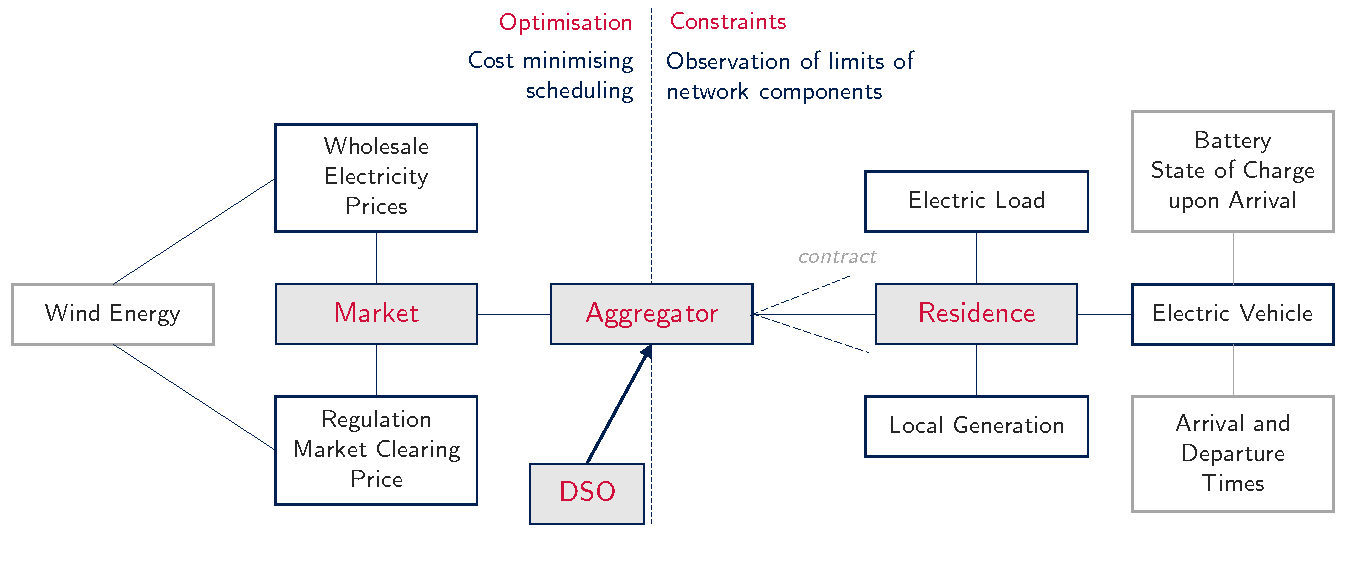
\includegraphics[scale = 0.48]{uncertainties.pdf}
	\end{figure}
\end{frame}

\subsection{Research Objectives}


\begin{frame}{Research Objectives}
	\textbf{Optimisation study based on a developed simulation model}\pause
	\begin{itemize}
		\item Develop a \textcolor{UOEyellow}{robust} \textcolor{UOEgreen}{cost-minimising} \textcolor{UOEblue2}{(bidirectional)} scheduling routine for charging EVs \textcolor{UOEred}{while observing network, equipment and demand constraints} \textcolor{UOEyellow}{in a stochastic environment}.\pause
		\item Characterise inherent and conceded uncertainties incurred with the optimal scheduling of EVs. \textcolor{UOEblue2}{(esp.\ driving behaviour)}\pause
		\item Compare and assess the performance of multiple optimisation methods under uncertainty and approaches to mitigate their sensitivity to prediction errors.
		\begin{itemize}
			\item greedy heuristic\tab \textcolor{UOEblue2}{(benchmark optimisation)}
			\item metaheuristics\tab \textcolor{UOEblue2}{(PSO or GA)}
			\item analytical\tab \textcolor{UOEblue2}{(linear approximation)}
		\end{itemize}
	\end{itemize}
\end{frame}

\subsection{Optimisation Problem Formulation}

\begin{frame}{Extract of Problem Formulation}
	\begin{restoretext}
		\scriptsize
		\begingroup
		
		\renewcommand*{\arraystretch}{1.5}
		\begin{equation*}
		\begin{array}{rrccclcl}
		\min_{\{P_{EV},\omega\}} & \multicolumn{5}{l}{C=\sum_{t=1}^T \sum_{k=1}^{K} \sum_{d=1}^{D} \quad \hat{\pi}_t \cdot \Delta t \cdot \pev \quad - \quad \rho \cdot \eta \cdot P^{EV}_{max} \cdot \lev } \\ \hline \pause
		\text{s.t.} &&& \left(1-\aev\right)\cdot \pev & = & 0 \\
		& 0 & \leq & \pev & \leq & P^{EV}_{max} \\
		& \beta_{min}\cdot B_{max} & \leq &  \hat{B}^{arr}_{k,d}+\sum_{t=1}^{T} \eta \cdot \pev \cdot \Delta t & \leq & B_{max} \\
		& \gamma_{min} \cdot B_{max} & \leq & \lev \cdot \left(\hat{B}^{arr}_{k,d} + \sum_{\tau = 1}^{t} \eta \cdot \pevc \cdot \Delta t\right) & \leq & B_{max} \\	
		& \Delta^{EV}_{max} & \leq & \left(\aev\cdot\aevb\right)\cdot\left(\pev-\pevb\right)& \leq & \Delta^{EV}_{max}\\ \hline  \pause
		\text{PF} & V_{min} & \leq & V_{k,d,t}^{bus} & \leq & V_{max} \\
		& 0 & \leq & S_t^X & \leq & S^X_{rated} \\
		& 0 & \leq & I_{\ell,t}^{line} & \leq & I_{\ell}^{max} \\ \hline \pause
		& \multicolumn{5}{l}{\forall k\in \{1\dots K\} \quad \forall d\in \{1\dots D\} \quad \forall t\in \{1\dots T\} \quad \forall \ell\in \{1\dots L\}} \\
		\end{array}
		\end{equation*}
		\endgroup
		\normalsize
	\end{restoretext}
	~\\
	\small \textcolor{UOEred}{Example:} With 50 vehicles, 24 hour optimisation horizon and 15 minute resolution, the problem has minimum $2\cdot50\cdot96=9600$ decision variables.
	\normalsize
\end{frame}

\section{Project Status}

\subsection{Data Acquisition}

\begin{frame}{Data Acquisition}
	\begin{columns}
		\begin{column}{5.5cm}
			\textcolor{UOEblue3}{Price time series}
			\begin{itemize}
				\item UKPX Reference Price Data
			\end{itemize}
			\textcolor{UOEpink}{Demand time series}
			\begin{itemize}
				\item CREST demand model
			\end{itemize}
			\textcolor{UOEorange}{Network topology}
			\begin{itemize}
				\item European LV test feeder
			\end{itemize}
			\textcolor{UOEgreen}{Mobility data}
			\begin{itemize}
				\item National Travel Survey
			\end{itemize}
			\textcolor{UOEyellow}{Other parameters}
			\begin{itemize}
				\item vehicle specifications
				\item charging equipment
				\item ...
			\end{itemize}
		\end{column}
		\begin{column}{5.5cm}
			\begin{figure}
				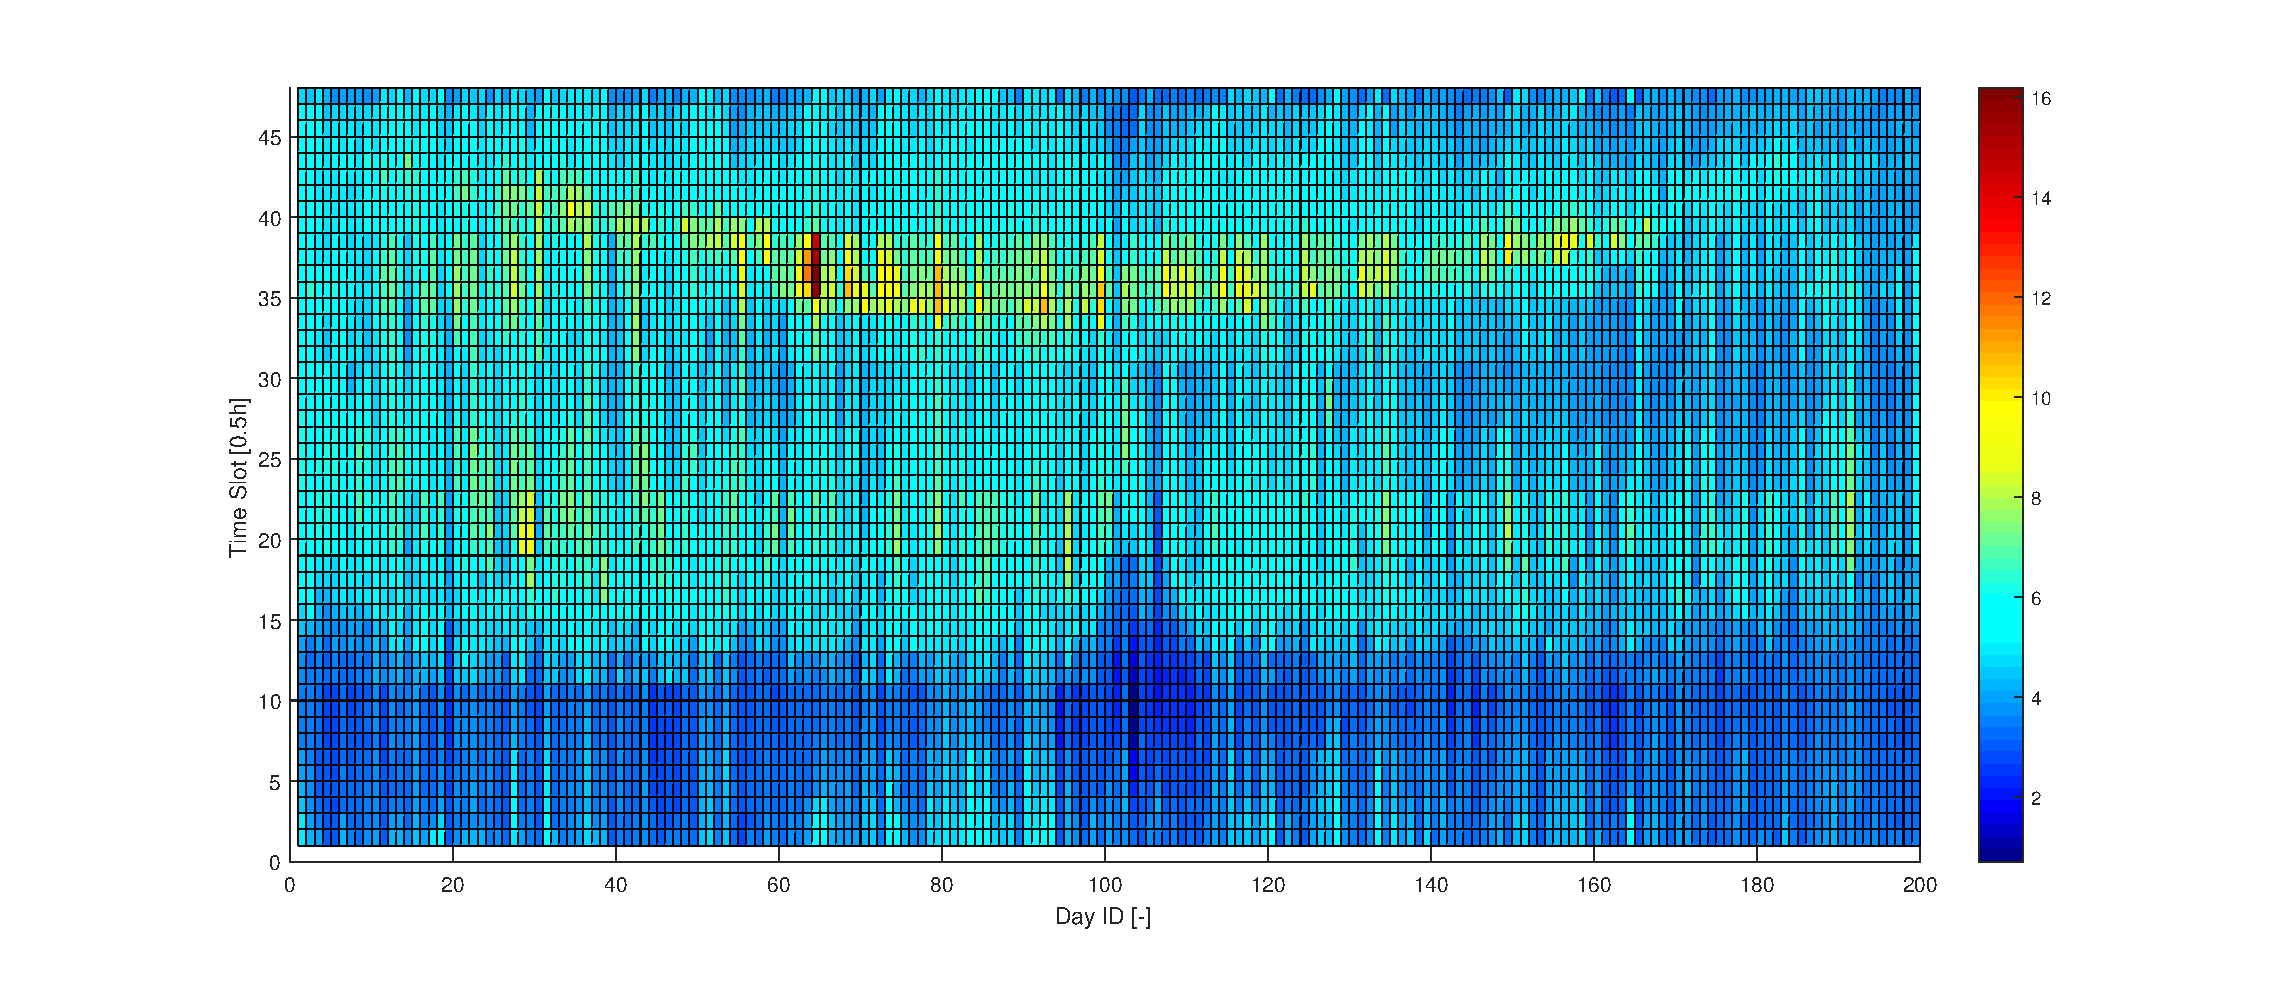
\includegraphics[trim={3cm 0.7cm 3cm 1cm},clip,scale = 0.18]{ukpx.eps}
			\end{figure}
			\begin{figure}
				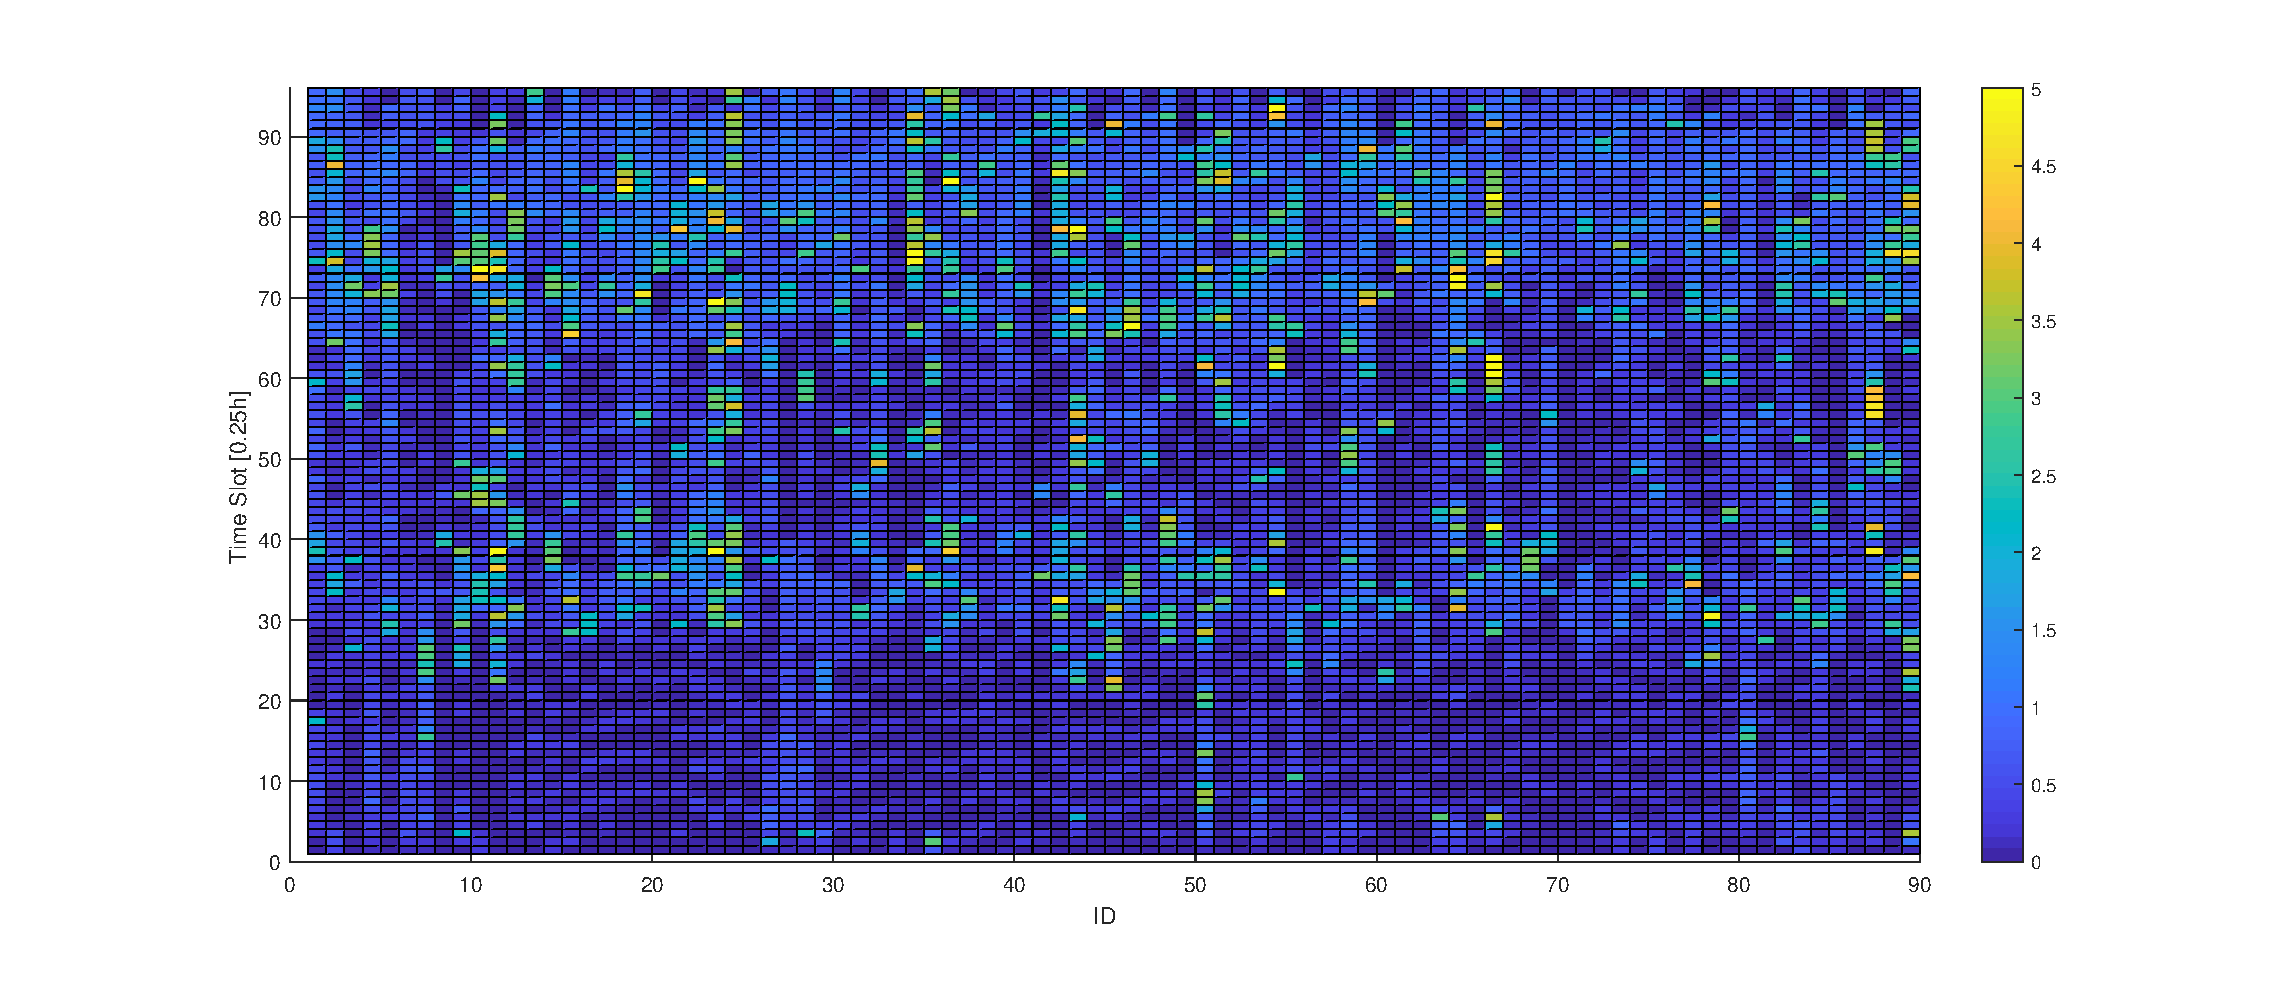
\includegraphics[trim={3cm 0.7cm 3cm 1cm},clip,scale = 0.18]{crest.eps}
			\end{figure}
		\end{column}
	\end{columns}
\end{frame}

\begin{frame}{Travel Pattern Analysis}
	\begin{figure}
		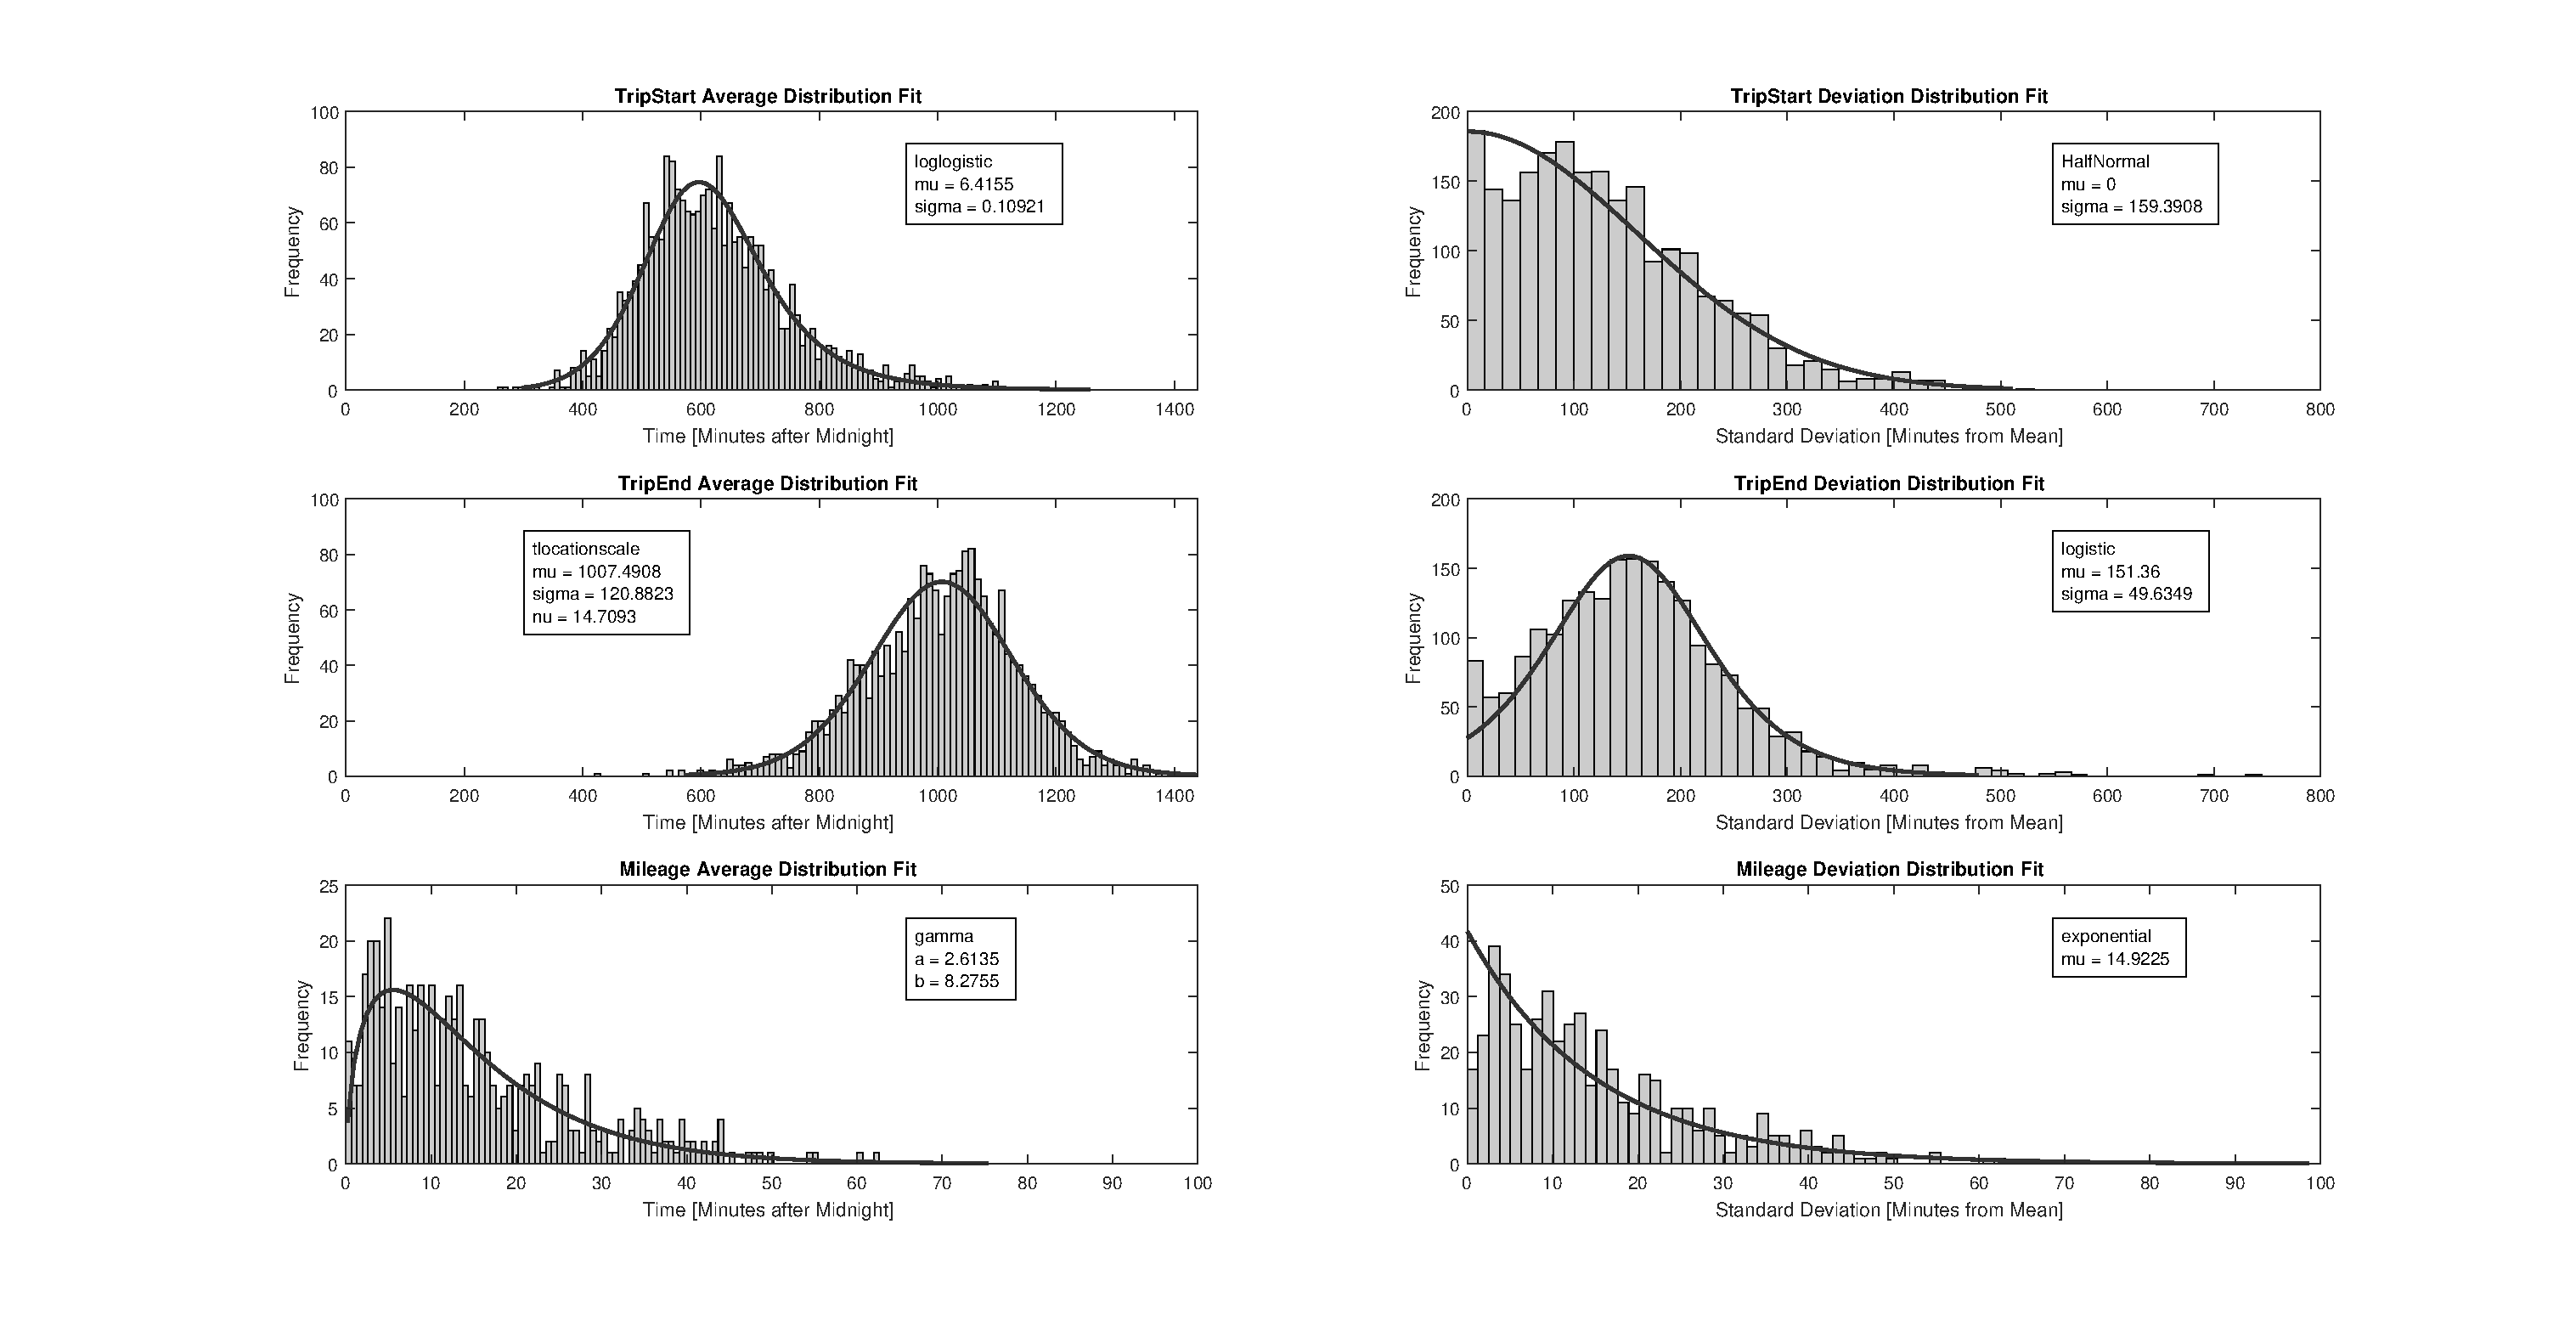
\includegraphics[trim={5.3cm 0cm 5.3cm 0cm},clip,scale = 0.28]{travelpatterns.eps}
	\end{figure}		
\end{frame}

\begin{frame}{Travel Pattern Analysis}
	\begin{figure}
		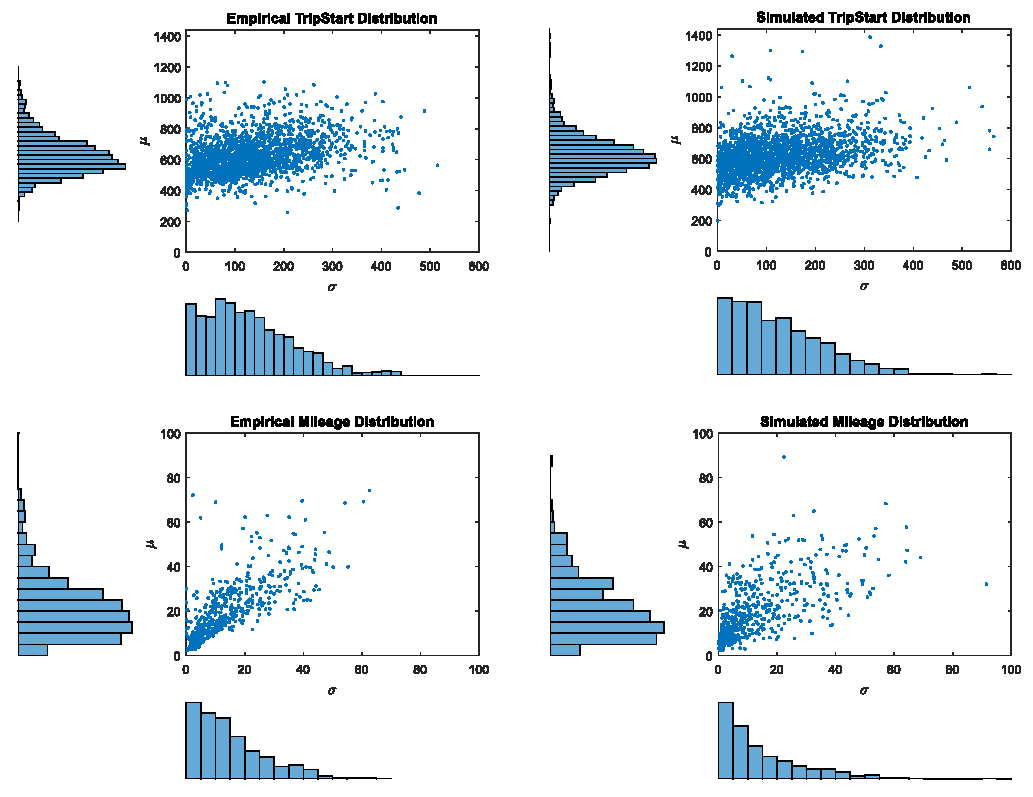
\includegraphics[scale = 0.55]{multivariate.pdf}
	\end{figure}		
\end{frame}

\subsection{Optimisation Routine}
\begin{frame}{Optimisation Routine}
	\begin{figure}
		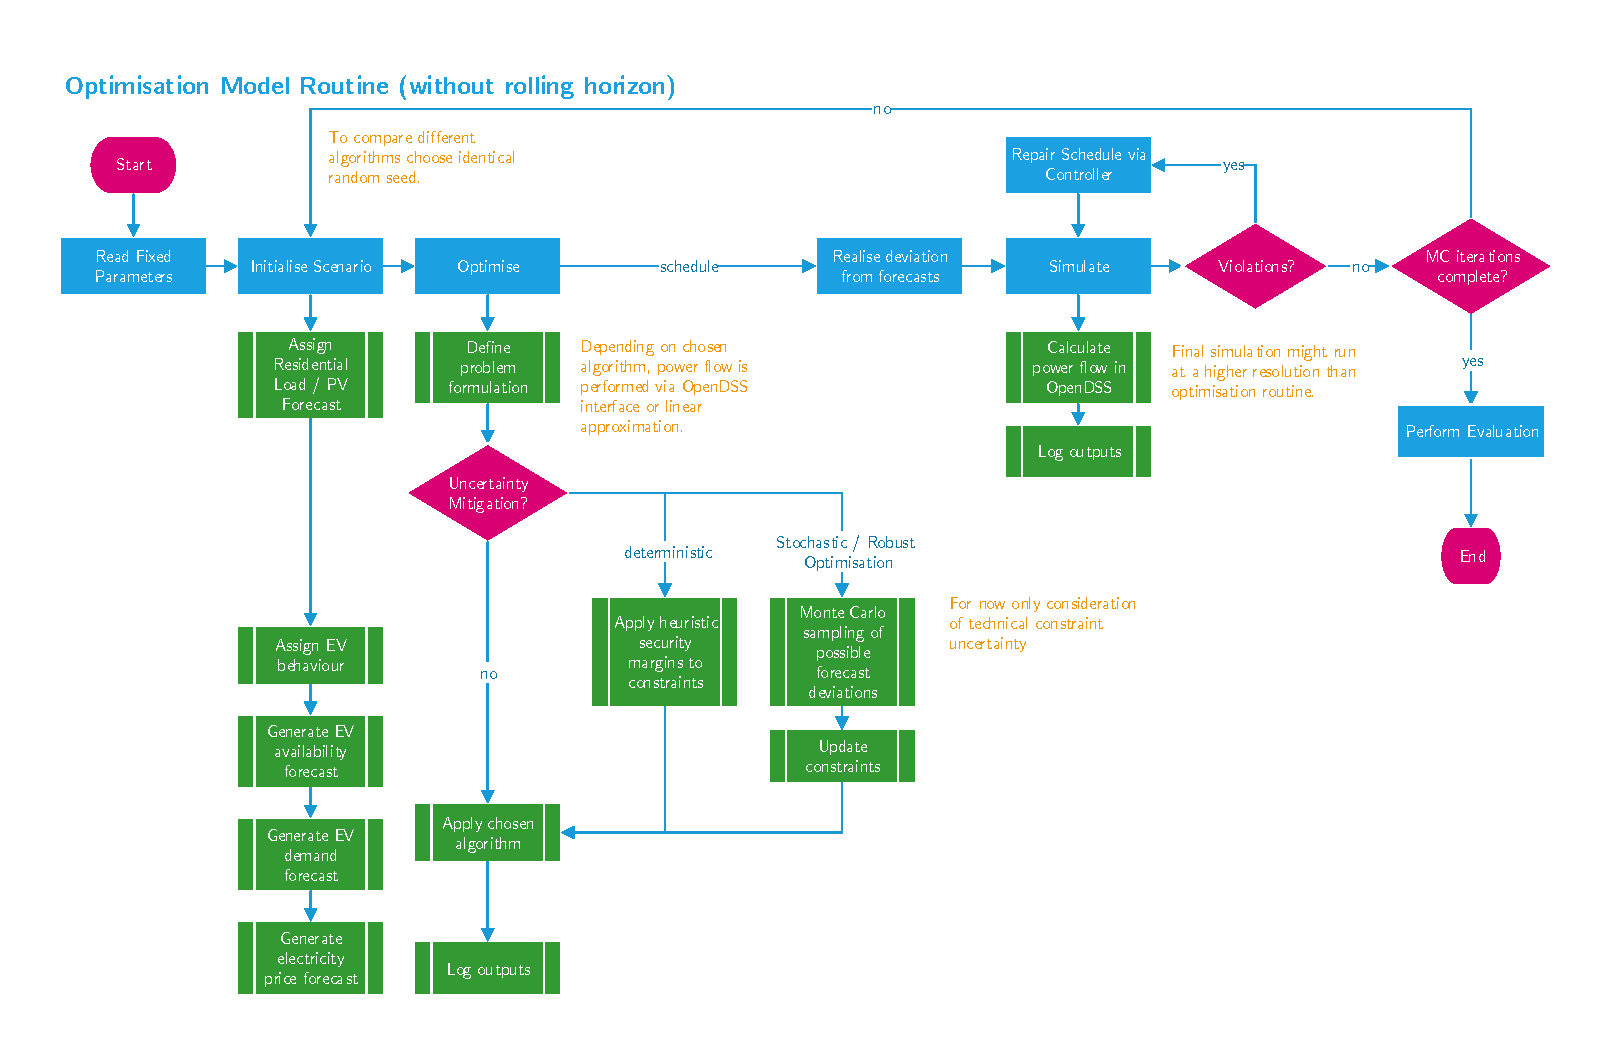
\includegraphics[trim={1cm 1cm 1cm 1cm},clip,width=1.07\linewidth]{optimisationroutine}
	\end{figure}		
\end{frame}

\section{Project Outlook}

\subsection*{What's next?}

\begin{frame}{Outlook on Upcoming Research}
	\begin{columns}[T]
		\begin{column}{6cm}
			\textcolor{UOEpink}{Implementation of...}
			\begin{itemize}
				\item optimisation/model framework \textcolor{UOEblue2}{(Python, OpenDSS)}
				\item optimisation algorithms
				\begin{itemize}
					\item greedy heuristic \textcolor{UOEblue2}{(manual)}
					\item GA/PSO \textcolor{UOEblue2}{(DEAP)}
					\item LP \textcolor{UOEblue2}{(Gurobi, approximation)}
				\end{itemize}
				\item uncertainty mitigation
				\begin{itemize}
					\item stochastic programming
					\item rolling optimisation horizon
				\end{itemize}
				\item reparation controller
			\end{itemize}
		\end{column}
	\pause
		\begin{column}{5.5cm}
			\textcolor{UOEgreen}{Anticipated Difficulties}
			\begin{itemize}
				\item thermal line limits data
				\item computational complexity
				\begin{itemize}
					\item decision variables
					\item power flow calculations
				\end{itemize}
				\item incorporation of ancillary services \textcolor{UOEblue2}{(market structure)}
				\item uncertainty modeling of demand, PV, and price
				\item information transfer and modelling forecast accuracy improvements \textcolor{UOEblue2}{(rolling opt.)}
				\item linear power flow approximation
			\end{itemize}
		\end{column}	
	\end{columns}
\end{frame}

% Placing a * after \section means it will not show in the
% outline or table of contents.
\section{Summary}

\subsection*{In a nutshell...}

\begin{frame}{Summary}
	\begin{columns}[T]
		\begin{column}{4.1cm}
			\textcolor{UOEpink}{Scheduling Problem}
			\begin{itemize}
				\item Cost Minimisation
				\item Physical Constraints
				\item Uncertainties
				\item 1-phase Connection
				\item Stochastic Programming
				\item Rolling Optimisation
			\end{itemize}
		\end{column}
	\pause
		\begin{column}{4cm}
			\textcolor{UOEgreen}{Done}
			\begin{itemize}
				\item Data Acquisition
				\item Travel Patterns
				\item Network Topology
				\item Parametrisation
				\item Power Flow in OpenDSS
			\end{itemize}
		\end{column}
	\pause
		\begin{column}{4cm}
			\textcolor{UOEyellow}{To Do}
			\begin{itemize}
				\item Framework Implementation
				\item Optimisation Algorithms
				\item Uncertainty Mitigation
				\item Real-time Controller
				\item Evaluation
				\item Write-up
			\end{itemize}
		\end{column}
	\end{columns}
\end{frame}



% All of the following is optional and typically not needed. 
%\appendix
%\section<presentation>*{\appendixname}
%\subsection<presentation>*{Bibliography}
%
%\begin{frame}[allowframebreaks]
%  \frametitle<presentation>{Bibliography}
%    
%  \begin{thebibliography}{10}
%    
%  \beamertemplatebookbibitems
%  % Start with overview books.
%
%  \bibitem{Author1990}
%    A.~Author.
%    \newblock {\em Handbook of Everything}.
%    \newblock Some Press, 1990.
% 
%    
%  \beamertemplatearticlebibitems
%  % Followed by interesting articles. Keep the list short. 
%
%  \bibitem{Someone2000}
%    S.~Someone.
%    \newblock On this and that.
%    \newblock {\em Journal of This and That}, 2(1):50--100,
%    2000.
%  \end{thebibliography}
%\end{frame}

\end{document}


